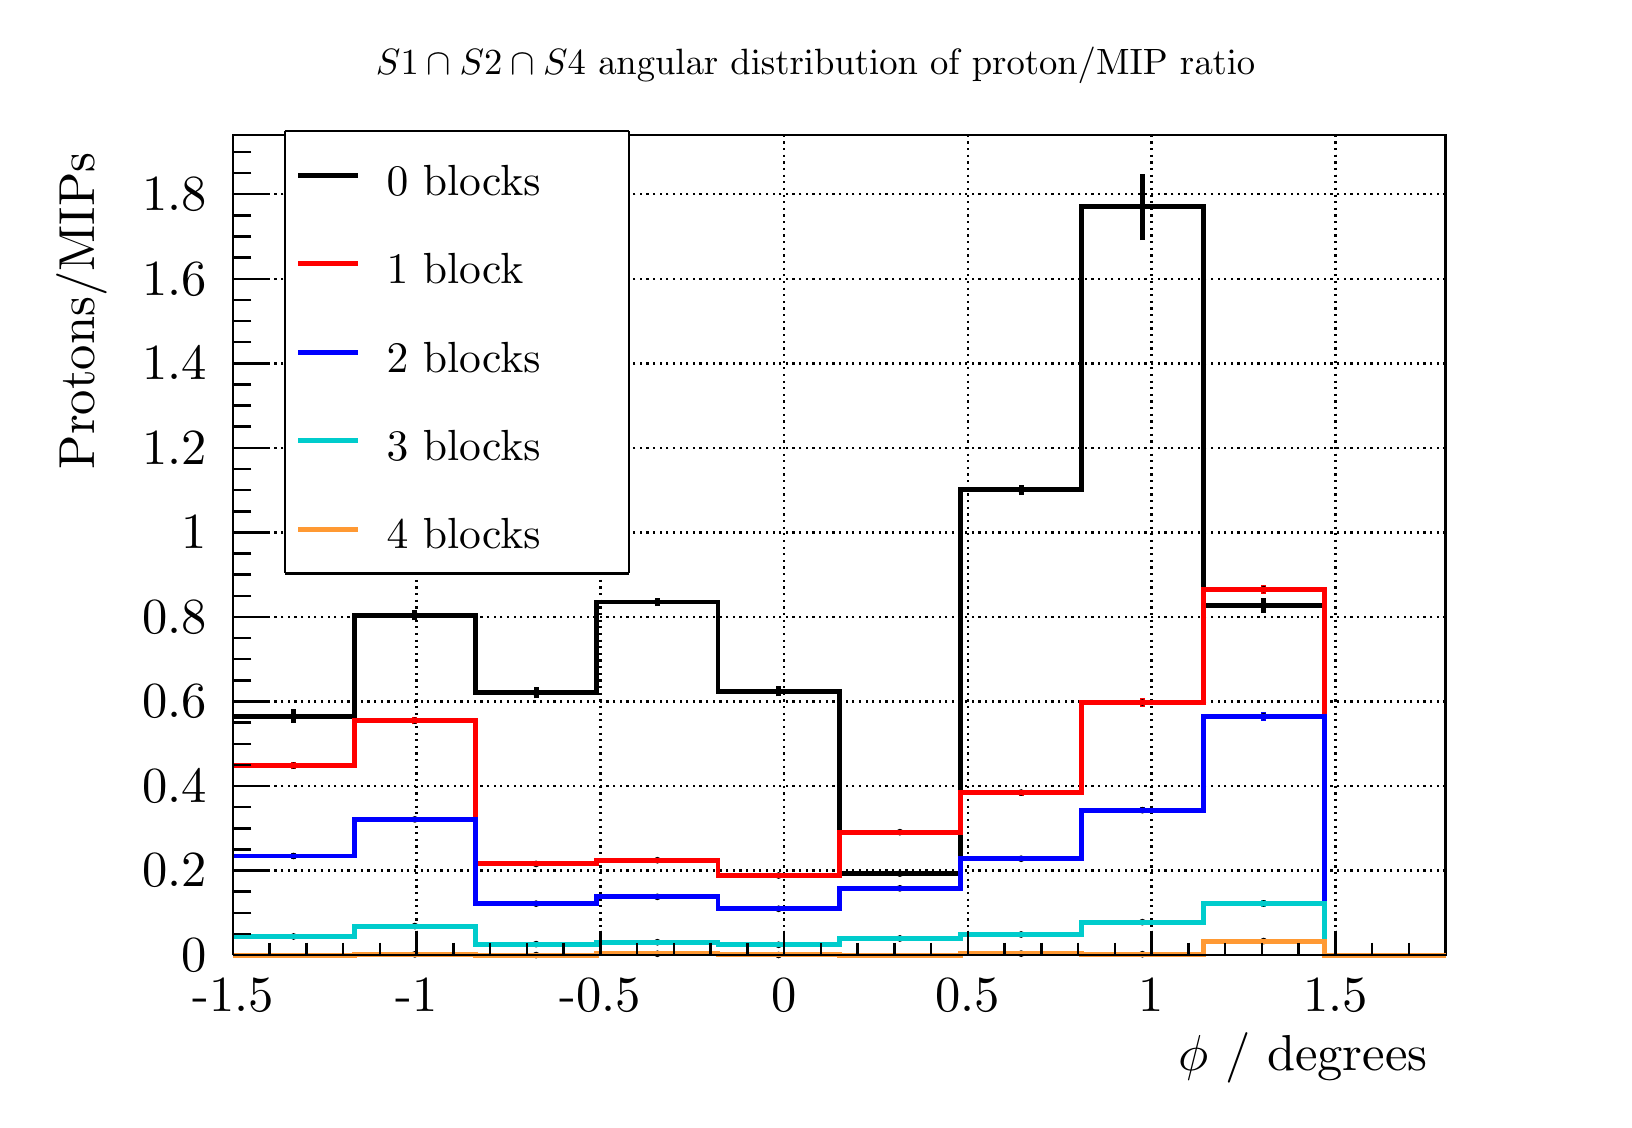
\begin{tikzpicture}
\pgfdeclareplotmark{cross} {
\pgfpathmoveto{\pgfpoint{-0.3\pgfplotmarksize}{\pgfplotmarksize}}
\pgfpathlineto{\pgfpoint{+0.3\pgfplotmarksize}{\pgfplotmarksize}}
\pgfpathlineto{\pgfpoint{+0.3\pgfplotmarksize}{0.3\pgfplotmarksize}}
\pgfpathlineto{\pgfpoint{+1\pgfplotmarksize}{0.3\pgfplotmarksize}}
\pgfpathlineto{\pgfpoint{+1\pgfplotmarksize}{-0.3\pgfplotmarksize}}
\pgfpathlineto{\pgfpoint{+0.3\pgfplotmarksize}{-0.3\pgfplotmarksize}}
\pgfpathlineto{\pgfpoint{+0.3\pgfplotmarksize}{-1.\pgfplotmarksize}}
\pgfpathlineto{\pgfpoint{-0.3\pgfplotmarksize}{-1.\pgfplotmarksize}}
\pgfpathlineto{\pgfpoint{-0.3\pgfplotmarksize}{-0.3\pgfplotmarksize}}
\pgfpathlineto{\pgfpoint{-1.\pgfplotmarksize}{-0.3\pgfplotmarksize}}
\pgfpathlineto{\pgfpoint{-1.\pgfplotmarksize}{0.3\pgfplotmarksize}}
\pgfpathlineto{\pgfpoint{-0.3\pgfplotmarksize}{0.3\pgfplotmarksize}}
\pgfpathclose
\pgfusepathqstroke
}
\pgfdeclareplotmark{cross*} {
\pgfpathmoveto{\pgfpoint{-0.3\pgfplotmarksize}{\pgfplotmarksize}}
\pgfpathlineto{\pgfpoint{+0.3\pgfplotmarksize}{\pgfplotmarksize}}
\pgfpathlineto{\pgfpoint{+0.3\pgfplotmarksize}{0.3\pgfplotmarksize}}
\pgfpathlineto{\pgfpoint{+1\pgfplotmarksize}{0.3\pgfplotmarksize}}
\pgfpathlineto{\pgfpoint{+1\pgfplotmarksize}{-0.3\pgfplotmarksize}}
\pgfpathlineto{\pgfpoint{+0.3\pgfplotmarksize}{-0.3\pgfplotmarksize}}
\pgfpathlineto{\pgfpoint{+0.3\pgfplotmarksize}{-1.\pgfplotmarksize}}
\pgfpathlineto{\pgfpoint{-0.3\pgfplotmarksize}{-1.\pgfplotmarksize}}
\pgfpathlineto{\pgfpoint{-0.3\pgfplotmarksize}{-0.3\pgfplotmarksize}}
\pgfpathlineto{\pgfpoint{-1.\pgfplotmarksize}{-0.3\pgfplotmarksize}}
\pgfpathlineto{\pgfpoint{-1.\pgfplotmarksize}{0.3\pgfplotmarksize}}
\pgfpathlineto{\pgfpoint{-0.3\pgfplotmarksize}{0.3\pgfplotmarksize}}
\pgfpathclose
\pgfusepathqfillstroke
}
\pgfdeclareplotmark{newstar} {
\pgfpathmoveto{\pgfqpoint{0pt}{\pgfplotmarksize}}
\pgfpathlineto{\pgfqpointpolar{44}{0.5\pgfplotmarksize}}
\pgfpathlineto{\pgfqpointpolar{18}{\pgfplotmarksize}}
\pgfpathlineto{\pgfqpointpolar{-20}{0.5\pgfplotmarksize}}
\pgfpathlineto{\pgfqpointpolar{-54}{\pgfplotmarksize}}
\pgfpathlineto{\pgfqpointpolar{-90}{0.5\pgfplotmarksize}}
\pgfpathlineto{\pgfqpointpolar{234}{\pgfplotmarksize}}
\pgfpathlineto{\pgfqpointpolar{198}{0.5\pgfplotmarksize}}
\pgfpathlineto{\pgfqpointpolar{162}{\pgfplotmarksize}}
\pgfpathlineto{\pgfqpointpolar{134}{0.5\pgfplotmarksize}}
\pgfpathclose
\pgfusepathqstroke
}
\pgfdeclareplotmark{newstar*} {
\pgfpathmoveto{\pgfqpoint{0pt}{\pgfplotmarksize}}
\pgfpathlineto{\pgfqpointpolar{44}{0.5\pgfplotmarksize}}
\pgfpathlineto{\pgfqpointpolar{18}{\pgfplotmarksize}}
\pgfpathlineto{\pgfqpointpolar{-20}{0.5\pgfplotmarksize}}
\pgfpathlineto{\pgfqpointpolar{-54}{\pgfplotmarksize}}
\pgfpathlineto{\pgfqpointpolar{-90}{0.5\pgfplotmarksize}}
\pgfpathlineto{\pgfqpointpolar{234}{\pgfplotmarksize}}
\pgfpathlineto{\pgfqpointpolar{198}{0.5\pgfplotmarksize}}
\pgfpathlineto{\pgfqpointpolar{162}{\pgfplotmarksize}}
\pgfpathlineto{\pgfqpointpolar{134}{0.5\pgfplotmarksize}}
\pgfpathclose
\pgfusepathqfillstroke
}
\definecolor{c}{rgb}{1,1,1};
\draw [color=c, fill=c] (0,0) rectangle (20,13.5319);
\draw [color=c, fill=c] (2.6,1.75915) rectangle (18,12.1787);
\definecolor{c}{rgb}{0,0,0};
\draw [c,line width=0.9] (2.6,1.75915) -- (2.6,12.1787) -- (18,12.1787) -- (18,1.75915) -- (2.6,1.75915);
\definecolor{c}{rgb}{1,1,1};
\draw [color=c, fill=c] (2.6,1.75915) rectangle (18,12.1787);
\definecolor{c}{rgb}{0,0,0};
\draw [c,line width=0.9] (2.6,1.75915) -- (2.6,12.1787) -- (18,12.1787) -- (18,1.75915) -- (2.6,1.75915);
\draw [c,line width=0.9] (2.6,1.75915) -- (18,1.75915);
\draw [c,dash pattern=on 0.80pt off 1.60pt ,line width=0.9] (2.6,12.1787) -- (2.6,1.75915);
\draw [c,dash pattern=on 0.80pt off 1.60pt ,line width=0.9] (4.93333,12.1787) -- (4.93333,1.75915);
\draw [c,dash pattern=on 0.80pt off 1.60pt ,line width=0.9] (7.26667,12.1787) -- (7.26667,1.75915);
\draw [c,dash pattern=on 0.80pt off 1.60pt ,line width=0.9] (9.6,12.1787) -- (9.6,1.75915);
\draw [c,dash pattern=on 0.80pt off 1.60pt ,line width=0.9] (11.9333,12.1787) -- (11.9333,1.75915);
\draw [c,dash pattern=on 0.80pt off 1.60pt ,line width=0.9] (14.2667,12.1787) -- (14.2667,1.75915);
\draw [c,dash pattern=on 0.80pt off 1.60pt ,line width=0.9] (16.6,12.1787) -- (16.6,1.75915);
\draw [c,dash pattern=on 0.80pt off 1.60pt ,line width=0.9] (16.6,12.1787) -- (16.6,1.75915);
\draw [c,line width=0.9] (2.6,1.75915) -- (2.6,12.1787);
\draw [c,dash pattern=on 0.80pt off 1.60pt ,line width=0.9] (18,1.76049) -- (2.6,1.76049);
\draw [c,dash pattern=on 0.80pt off 1.60pt ,line width=0.9] (18,2.83413) -- (2.6,2.83413);
\draw [c,dash pattern=on 0.80pt off 1.60pt ,line width=0.9] (18,3.90776) -- (2.6,3.90776);
\draw [c,dash pattern=on 0.80pt off 1.60pt ,line width=0.9] (18,4.98139) -- (2.6,4.98139);
\draw [c,dash pattern=on 0.80pt off 1.60pt ,line width=0.9] (18,6.05503) -- (2.6,6.05503);
\draw [c,dash pattern=on 0.80pt off 1.60pt ,line width=0.9] (18,7.12866) -- (2.6,7.12866);
\draw [c,dash pattern=on 0.80pt off 1.60pt ,line width=0.9] (18,8.20229) -- (2.6,8.20229);
\draw [c,dash pattern=on 0.80pt off 1.60pt ,line width=0.9] (18,9.27592) -- (2.6,9.27592);
\draw [c,dash pattern=on 0.80pt off 1.60pt ,line width=0.9] (18,10.3496) -- (2.6,10.3496);
\draw [c,dash pattern=on 0.80pt off 1.60pt ,line width=0.9] (18,11.4232) -- (2.6,11.4232);
\draw [c,dash pattern=on 0.80pt off 1.60pt ,line width=0.9] (18,1.76049) -- (2.6,1.76049);
\draw [c,dash pattern=on 0.80pt off 1.60pt ,line width=0.9] (18,11.4232) -- (2.6,11.4232);
\definecolor{c}{rgb}{0,0,0.6};
\draw [c,line width=0.9] (2.6,1.76049) -- (4.14,1.76049) -- (4.14,1.76049) -- (5.68,1.76049) -- (5.68,1.76049) -- (7.22,1.76049) -- (7.22,1.76049) -- (8.76,1.76049) -- (8.76,1.76049) -- (10.3,1.76049) -- (10.3,1.76049) -- (11.84,1.76049) --
 (11.84,1.76049) -- (13.38,1.76049) -- (13.38,1.76049) -- (14.92,1.76049) -- (14.92,1.76049) -- (16.46,1.76049) -- (16.46,1.76049) -- (18,1.76049);
\definecolor{c}{rgb}{0,0,0};
\draw [c,line width=0.9] (2.6,1.75915) -- (18,1.75915);
\draw [c,line width=0.9] (2.6,2.07174) -- (2.6,1.75915);
\draw [c,line width=0.9] (3.06667,1.91544) -- (3.06667,1.75915);
\draw [c,line width=0.9] (3.53333,1.91544) -- (3.53333,1.75915);
\draw [c,line width=0.9] (4,1.91544) -- (4,1.75915);
\draw [c,line width=0.9] (4.46667,1.91544) -- (4.46667,1.75915);
\draw [c,line width=0.9] (4.93333,2.07174) -- (4.93333,1.75915);
\draw [c,line width=0.9] (5.4,1.91544) -- (5.4,1.75915);
\draw [c,line width=0.9] (5.86667,1.91544) -- (5.86667,1.75915);
\draw [c,line width=0.9] (6.33333,1.91544) -- (6.33333,1.75915);
\draw [c,line width=0.9] (6.8,1.91544) -- (6.8,1.75915);
\draw [c,line width=0.9] (7.26667,2.07174) -- (7.26667,1.75915);
\draw [c,line width=0.9] (7.73333,1.91544) -- (7.73333,1.75915);
\draw [c,line width=0.9] (8.2,1.91544) -- (8.2,1.75915);
\draw [c,line width=0.9] (8.66667,1.91544) -- (8.66667,1.75915);
\draw [c,line width=0.9] (9.13333,1.91544) -- (9.13333,1.75915);
\draw [c,line width=0.9] (9.6,2.07174) -- (9.6,1.75915);
\draw [c,line width=0.9] (10.0667,1.91544) -- (10.0667,1.75915);
\draw [c,line width=0.9] (10.5333,1.91544) -- (10.5333,1.75915);
\draw [c,line width=0.9] (11,1.91544) -- (11,1.75915);
\draw [c,line width=0.9] (11.4667,1.91544) -- (11.4667,1.75915);
\draw [c,line width=0.9] (11.9333,2.07174) -- (11.9333,1.75915);
\draw [c,line width=0.9] (12.4,1.91544) -- (12.4,1.75915);
\draw [c,line width=0.9] (12.8667,1.91544) -- (12.8667,1.75915);
\draw [c,line width=0.9] (13.3333,1.91544) -- (13.3333,1.75915);
\draw [c,line width=0.9] (13.8,1.91544) -- (13.8,1.75915);
\draw [c,line width=0.9] (14.2667,2.07174) -- (14.2667,1.75915);
\draw [c,line width=0.9] (14.7333,1.91544) -- (14.7333,1.75915);
\draw [c,line width=0.9] (15.2,1.91544) -- (15.2,1.75915);
\draw [c,line width=0.9] (15.6667,1.91544) -- (15.6667,1.75915);
\draw [c,line width=0.9] (16.1333,1.91544) -- (16.1333,1.75915);
\draw [c,line width=0.9] (16.6,2.07174) -- (16.6,1.75915);
\draw [c,line width=0.9] (16.6,2.07174) -- (16.6,1.75915);
\draw [c,line width=0.9] (17.0667,1.91544) -- (17.0667,1.75915);
\draw [c,line width=0.9] (17.5333,1.91544) -- (17.5333,1.75915);
\draw [anchor=base] (2.6,1.04196) node[scale=1.82718, color=c, rotate=0]{-1.5};
\draw [anchor=base] (4.93333,1.04196) node[scale=1.82718, color=c, rotate=0]{-1};
\draw [anchor=base] (7.26667,1.04196) node[scale=1.82718, color=c, rotate=0]{-0.5};
\draw [anchor=base] (9.6,1.04196) node[scale=1.82718, color=c, rotate=0]{0};
\draw [anchor=base] (11.9333,1.04196) node[scale=1.82718, color=c, rotate=0]{0.5};
\draw [anchor=base] (14.2667,1.04196) node[scale=1.82718, color=c, rotate=0]{1};
\draw [anchor=base] (16.6,1.04196) node[scale=1.82718, color=c, rotate=0]{1.5};
\draw [anchor= east] (18,0.460085) node[scale=1.82718, color=c, rotate=0]{$\phi$ / degrees};
\draw [c,line width=0.9] (2.6,1.75915) -- (2.6,12.1787);
\draw [c,line width=0.9] (3.062,1.76049) -- (2.6,1.76049);
\draw [c,line width=0.9] (2.831,2.0289) -- (2.6,2.0289);
\draw [c,line width=0.9] (2.831,2.29731) -- (2.6,2.29731);
\draw [c,line width=0.9] (2.831,2.56572) -- (2.6,2.56572);
\draw [c,line width=0.9] (3.062,2.83413) -- (2.6,2.83413);
\draw [c,line width=0.9] (2.831,3.10254) -- (2.6,3.10254);
\draw [c,line width=0.9] (2.831,3.37094) -- (2.6,3.37094);
\draw [c,line width=0.9] (2.831,3.63935) -- (2.6,3.63935);
\draw [c,line width=0.9] (3.062,3.90776) -- (2.6,3.90776);
\draw [c,line width=0.9] (2.831,4.17617) -- (2.6,4.17617);
\draw [c,line width=0.9] (2.831,4.44458) -- (2.6,4.44458);
\draw [c,line width=0.9] (2.831,4.71299) -- (2.6,4.71299);
\draw [c,line width=0.9] (3.062,4.98139) -- (2.6,4.98139);
\draw [c,line width=0.9] (2.831,5.2498) -- (2.6,5.2498);
\draw [c,line width=0.9] (2.831,5.51821) -- (2.6,5.51821);
\draw [c,line width=0.9] (2.831,5.78662) -- (2.6,5.78662);
\draw [c,line width=0.9] (3.062,6.05503) -- (2.6,6.05503);
\draw [c,line width=0.9] (2.831,6.32343) -- (2.6,6.32343);
\draw [c,line width=0.9] (2.831,6.59184) -- (2.6,6.59184);
\draw [c,line width=0.9] (2.831,6.86025) -- (2.6,6.86025);
\draw [c,line width=0.9] (3.062,7.12866) -- (2.6,7.12866);
\draw [c,line width=0.9] (2.831,7.39707) -- (2.6,7.39707);
\draw [c,line width=0.9] (2.831,7.66548) -- (2.6,7.66548);
\draw [c,line width=0.9] (2.831,7.93388) -- (2.6,7.93388);
\draw [c,line width=0.9] (3.062,8.20229) -- (2.6,8.20229);
\draw [c,line width=0.9] (2.831,8.4707) -- (2.6,8.4707);
\draw [c,line width=0.9] (2.831,8.73911) -- (2.6,8.73911);
\draw [c,line width=0.9] (2.831,9.00752) -- (2.6,9.00752);
\draw [c,line width=0.9] (3.062,9.27592) -- (2.6,9.27592);
\draw [c,line width=0.9] (2.831,9.54433) -- (2.6,9.54433);
\draw [c,line width=0.9] (2.831,9.81274) -- (2.6,9.81274);
\draw [c,line width=0.9] (2.831,10.0812) -- (2.6,10.0812);
\draw [c,line width=0.9] (3.062,10.3496) -- (2.6,10.3496);
\draw [c,line width=0.9] (2.831,10.618) -- (2.6,10.618);
\draw [c,line width=0.9] (2.831,10.8864) -- (2.6,10.8864);
\draw [c,line width=0.9] (2.831,11.1548) -- (2.6,11.1548);
\draw [c,line width=0.9] (3.062,11.4232) -- (2.6,11.4232);
\draw [c,line width=0.9] (3.062,1.76049) -- (2.6,1.76049);
\draw [c,line width=0.9] (3.062,11.4232) -- (2.6,11.4232);
\draw [c,line width=0.9] (2.831,11.6916) -- (2.6,11.6916);
\draw [c,line width=0.9] (2.831,11.96) -- (2.6,11.96);
\draw [anchor= east] (2.5,1.76049) node[scale=1.82718, color=c, rotate=0]{0};
\draw [anchor= east] (2.5,2.83413) node[scale=1.82718, color=c, rotate=0]{0.2};
\draw [anchor= east] (2.5,3.90776) node[scale=1.82718, color=c, rotate=0]{0.4};
\draw [anchor= east] (2.5,4.98139) node[scale=1.82718, color=c, rotate=0]{0.6};
\draw [anchor= east] (2.5,6.05503) node[scale=1.82718, color=c, rotate=0]{0.8};
\draw [anchor= east] (2.5,7.12866) node[scale=1.82718, color=c, rotate=0]{1};
\draw [anchor= east] (2.5,8.20229) node[scale=1.82718, color=c, rotate=0]{1.2};
\draw [anchor= east] (2.5,9.27592) node[scale=1.82718, color=c, rotate=0]{1.4};
\draw [anchor= east] (2.5,10.3496) node[scale=1.82718, color=c, rotate=0]{1.6};
\draw [anchor= east] (2.5,11.4232) node[scale=1.82718, color=c, rotate=0]{1.8};
\draw [anchor= east] (0.68,12.1787) node[scale=1.82718, color=c, rotate=90]{ Protons/MIPs};
\draw [c,line width=1.8] (3.37,4.71025) -- (3.37,4.79585);
\draw [c,line width=1.8] (3.37,4.79585) -- (3.37,4.88144);
\foreach \P in {(3.37,4.79585)}{\draw[mark options={color=c,fill=c},mark size=2.402402pt,mark=*,mark size=1pt] plot coordinates {\P};}
\draw [c,line width=1.8] (4.91,6.01214) -- (4.91,6.07843);
\draw [c,line width=1.8] (4.91,6.07843) -- (4.91,6.14473);
\foreach \P in {(4.91,6.07843)}{\draw[mark options={color=c,fill=c},mark size=2.402402pt,mark=*,mark size=1pt] plot coordinates {\P};}
\draw [c,line width=1.8] (6.45,5.02108) -- (6.45,5.09041);
\draw [c,line width=1.8] (6.45,5.09041) -- (6.45,5.15974);
\foreach \P in {(6.45,5.09041)}{\draw[mark options={color=c,fill=c},mark size=2.402402pt,mark=*,mark size=1pt] plot coordinates {\P};}
\draw [c,line width=1.8] (7.99,6.19173) -- (7.99,6.24488);
\draw [c,line width=1.8] (7.99,6.24488) -- (7.99,6.29803);
\foreach \P in {(7.99,6.24488)}{\draw[mark options={color=c,fill=c},mark size=2.402402pt,mark=*,mark size=1pt] plot coordinates {\P};}
\draw [c,line width=1.8] (9.53,5.0449) -- (9.53,5.10882);
\draw [c,line width=1.8] (9.53,5.10882) -- (9.53,5.17273);
\foreach \P in {(9.53,5.10882)}{\draw[mark options={color=c,fill=c},mark size=2.402402pt,mark=*,mark size=1pt] plot coordinates {\P};}
\draw [c,line width=1.8] (11.07,2.76645) -- (11.07,2.79547);
\draw [c,line width=1.8] (11.07,2.79547) -- (11.07,2.82449);
\foreach \P in {(11.07,2.79547)}{\draw[mark options={color=c,fill=c},mark size=2.402402pt,mark=*,mark size=1pt] plot coordinates {\P};}
\draw [c,line width=1.8] (12.61,7.60244) -- (12.61,7.66965);
\draw [c,line width=1.8] (12.61,7.66965) -- (12.61,7.73685);
\foreach \P in {(12.61,7.66965)}{\draw[mark options={color=c,fill=c},mark size=2.402402pt,mark=*,mark size=1pt] plot coordinates {\P};}
\draw [c,line width=1.8] (14.15,10.8412) -- (14.15,11.2619);
\draw [c,line width=1.8] (14.15,11.2619) -- (14.15,11.6826);
\foreach \P in {(14.15,11.2619)}{\draw[mark options={color=c,fill=c},mark size=2.402402pt,mark=*,mark size=1pt] plot coordinates {\P};}
\draw [c,line width=1.8] (15.69,6.11068) -- (15.69,6.20631);
\draw [c,line width=1.8] (15.69,6.20631) -- (15.69,6.30194);
\foreach \P in {(15.69,6.20631)}{\draw[mark options={color=c,fill=c},mark size=2.402402pt,mark=*,mark size=1pt] plot coordinates {\P};}
\draw [c,line width=1.8] (2.6,4.79585) -- (4.14,4.79585) -- (4.14,6.07843) -- (5.68,6.07843) -- (5.68,5.09041) -- (7.22,5.09041) -- (7.22,6.24488) -- (8.76,6.24488) -- (8.76,5.10882) -- (10.3,5.10882) -- (10.3,2.79547) -- (11.84,2.79547) --
 (11.84,7.66965) -- (13.38,7.66965) -- (13.38,11.2619) -- (14.92,11.2619) -- (14.92,6.20631) -- (16.46,6.20631) -- (16.46,1.76049) -- (18,1.76049);
\definecolor{c}{rgb}{1,0,0};
\draw [c,line width=1.8] (3.37,4.11807) -- (3.37,4.16704);
\draw [c,line width=1.8] (3.37,4.16704) -- (3.37,4.21602);
\definecolor{c}{rgb}{0,0,0};
\foreach \P in {(3.37,4.16704)}{\draw[mark options={color=c,fill=c},mark size=2.402402pt,mark=*,mark size=1pt] plot coordinates {\P};}
\definecolor{c}{rgb}{1,0,0};
\draw [c,line width=1.8] (4.91,4.69191) -- (4.91,4.73817);
\draw [c,line width=1.8] (4.91,4.73817) -- (4.91,4.78443);
\definecolor{c}{rgb}{0,0,0};
\foreach \P in {(4.91,4.73817)}{\draw[mark options={color=c,fill=c},mark size=2.402402pt,mark=*,mark size=1pt] plot coordinates {\P};}
\definecolor{c}{rgb}{1,0,0};
\draw [c,line width=1.8] (6.45,2.89584) -- (6.45,2.91871);
\draw [c,line width=1.8] (6.45,2.91871) -- (6.45,2.94158);
\definecolor{c}{rgb}{0,0,0};
\foreach \P in {(6.45,2.91871)}{\draw[mark options={color=c,fill=c},mark size=2.402402pt,mark=*,mark size=1pt] plot coordinates {\P};}
\definecolor{c}{rgb}{1,0,0};
\draw [c,line width=1.8] (7.99,2.94378) -- (7.99,2.96547);
\draw [c,line width=1.8] (7.99,2.96547) -- (7.99,2.98716);
\definecolor{c}{rgb}{0,0,0};
\foreach \P in {(7.99,2.96547)}{\draw[mark options={color=c,fill=c},mark size=2.402402pt,mark=*,mark size=1pt] plot coordinates {\P};}
\definecolor{c}{rgb}{1,0,0};
\draw [c,line width=1.8] (9.53,2.75198) -- (9.53,2.7712);
\draw [c,line width=1.8] (9.53,2.7712) -- (9.53,2.79042);
\definecolor{c}{rgb}{0,0,0};
\foreach \P in {(9.53,2.7712)}{\draw[mark options={color=c,fill=c},mark size=2.402402pt,mark=*,mark size=1pt] plot coordinates {\P};}
\definecolor{c}{rgb}{1,0,0};
\draw [c,line width=1.8] (11.07,3.29511) -- (11.07,3.32202);
\draw [c,line width=1.8] (11.07,3.32202) -- (11.07,3.34893);
\definecolor{c}{rgb}{0,0,0};
\foreach \P in {(11.07,3.32202)}{\draw[mark options={color=c,fill=c},mark size=2.402402pt,mark=*,mark size=1pt] plot coordinates {\P};}
\definecolor{c}{rgb}{1,0,0};
\draw [c,line width=1.8] (12.61,3.78663) -- (12.61,3.8247);
\draw [c,line width=1.8] (12.61,3.8247) -- (12.61,3.86278);
\definecolor{c}{rgb}{0,0,0};
\foreach \P in {(12.61,3.8247)}{\draw[mark options={color=c,fill=c},mark size=2.402402pt,mark=*,mark size=1pt] plot coordinates {\P};}
\definecolor{c}{rgb}{1,0,0};
\draw [c,line width=1.8] (14.15,4.91557) -- (14.15,4.96824);
\draw [c,line width=1.8] (14.15,4.96824) -- (14.15,5.02092);
\definecolor{c}{rgb}{0,0,0};
\foreach \P in {(14.15,4.96824)}{\draw[mark options={color=c,fill=c},mark size=2.402402pt,mark=*,mark size=1pt] plot coordinates {\P};}
\definecolor{c}{rgb}{1,0,0};
\draw [c,line width=1.8] (15.69,6.35074) -- (15.69,6.40782);
\draw [c,line width=1.8] (15.69,6.40782) -- (15.69,6.46491);
\definecolor{c}{rgb}{0,0,0};
\foreach \P in {(15.69,6.40782)}{\draw[mark options={color=c,fill=c},mark size=2.402402pt,mark=*,mark size=1pt] plot coordinates {\P};}
\definecolor{c}{rgb}{1,0,0};
\draw [c,line width=1.8] (2.6,4.16704) -- (4.14,4.16704) -- (4.14,4.73817) -- (5.68,4.73817) -- (5.68,2.91871) -- (7.22,2.91871) -- (7.22,2.96547) -- (8.76,2.96547) -- (8.76,2.7712) -- (10.3,2.7712) -- (10.3,3.32202) -- (11.84,3.32202) --
 (11.84,3.8247) -- (13.38,3.8247) -- (13.38,4.96824) -- (14.92,4.96824) -- (14.92,6.40782) -- (16.46,6.40782) -- (16.46,1.76049) -- (18,1.76049);
\definecolor{c}{rgb}{0,0,1};
\draw [c,line width=1.8] (3.37,2.98714) -- (3.37,3.01918);
\draw [c,line width=1.8] (3.37,3.01918) -- (3.37,3.05122);
\definecolor{c}{rgb}{0,0,0};
\foreach \P in {(3.37,3.01918)}{\draw[mark options={color=c,fill=c},mark size=2.402402pt,mark=*,mark size=1pt] plot coordinates {\P};}
\definecolor{c}{rgb}{0,0,1};
\draw [c,line width=1.8] (4.91,3.45069) -- (4.91,3.48427);
\draw [c,line width=1.8] (4.91,3.48427) -- (4.91,3.51785);
\definecolor{c}{rgb}{0,0,0};
\foreach \P in {(4.91,3.48427)}{\draw[mark options={color=c,fill=c},mark size=2.402402pt,mark=*,mark size=1pt] plot coordinates {\P};}
\definecolor{c}{rgb}{0,0,1};
\draw [c,line width=1.8] (6.45,2.39914) -- (6.45,2.41346);
\draw [c,line width=1.8] (6.45,2.41346) -- (6.45,2.42778);
\definecolor{c}{rgb}{0,0,0};
\foreach \P in {(6.45,2.41346)}{\draw[mark options={color=c,fill=c},mark size=2.402402pt,mark=*,mark size=1pt] plot coordinates {\P};}
\definecolor{c}{rgb}{0,0,1};
\draw [c,line width=1.8] (7.99,2.48633) -- (7.99,2.50057);
\draw [c,line width=1.8] (7.99,2.50057) -- (7.99,2.51481);
\definecolor{c}{rgb}{0,0,0};
\foreach \P in {(7.99,2.50057)}{\draw[mark options={color=c,fill=c},mark size=2.402402pt,mark=*,mark size=1pt] plot coordinates {\P};}
\definecolor{c}{rgb}{0,0,1};
\draw [c,line width=1.8] (9.53,2.33638) -- (9.53,2.34859);
\draw [c,line width=1.8] (9.53,2.34859) -- (9.53,2.36079);
\definecolor{c}{rgb}{0,0,0};
\foreach \P in {(9.53,2.34859)}{\draw[mark options={color=c,fill=c},mark size=2.402402pt,mark=*,mark size=1pt] plot coordinates {\P};}
\definecolor{c}{rgb}{0,0,1};
\draw [c,line width=1.8] (11.07,2.5915) -- (11.07,2.60865);
\draw [c,line width=1.8] (11.07,2.60865) -- (11.07,2.6258);
\definecolor{c}{rgb}{0,0,0};
\foreach \P in {(11.07,2.60865)}{\draw[mark options={color=c,fill=c},mark size=2.402402pt,mark=*,mark size=1pt] plot coordinates {\P};}
\definecolor{c}{rgb}{0,0,1};
\draw [c,line width=1.8] (12.61,2.9584) -- (12.61,2.98436);
\draw [c,line width=1.8] (12.61,2.98436) -- (12.61,3.01032);
\definecolor{c}{rgb}{0,0,0};
\foreach \P in {(12.61,2.98436)}{\draw[mark options={color=c,fill=c},mark size=2.402402pt,mark=*,mark size=1pt] plot coordinates {\P};}
\definecolor{c}{rgb}{0,0,1};
\draw [c,line width=1.8] (14.15,3.56279) -- (14.15,3.60081);
\draw [c,line width=1.8] (14.15,3.60081) -- (14.15,3.63884);
\definecolor{c}{rgb}{0,0,0};
\foreach \P in {(14.15,3.60081)}{\draw[mark options={color=c,fill=c},mark size=2.402402pt,mark=*,mark size=1pt] plot coordinates {\P};}
\definecolor{c}{rgb}{0,0,1};
\draw [c,line width=1.8] (15.69,4.73566) -- (15.69,4.79491);
\draw [c,line width=1.8] (15.69,4.79491) -- (15.69,4.85415);
\definecolor{c}{rgb}{0,0,0};
\foreach \P in {(15.69,4.79491)}{\draw[mark options={color=c,fill=c},mark size=2.402402pt,mark=*,mark size=1pt] plot coordinates {\P};}
\definecolor{c}{rgb}{0,0,1};
\draw [c,line width=1.8] (2.6,3.01918) -- (4.14,3.01918) -- (4.14,3.48427) -- (5.68,3.48427) -- (5.68,2.41346) -- (7.22,2.41346) -- (7.22,2.50057) -- (8.76,2.50057) -- (8.76,2.34859) -- (10.3,2.34859) -- (10.3,2.60865) -- (11.84,2.60865) --
 (11.84,2.98436) -- (13.38,2.98436) -- (13.38,3.60081) -- (14.92,3.60081) -- (14.92,4.79491) -- (16.46,4.79491) -- (16.46,1.76049) -- (18,1.76049);
\definecolor{c}{rgb}{0,0.8,0.8};
\draw [c,line width=1.8] (3.37,1.9798) -- (3.37,1.9972);
\draw [c,line width=1.8] (3.37,1.9972) -- (3.37,2.0146);
\definecolor{c}{rgb}{0,0,0};
\foreach \P in {(3.37,1.9972)}{\draw[mark options={color=c,fill=c},mark size=2.402402pt,mark=*,mark size=1pt] plot coordinates {\P};}
\definecolor{c}{rgb}{0,0.8,0.8};
\draw [c,line width=1.8] (4.91,2.10989) -- (4.91,2.12941);
\draw [c,line width=1.8] (4.91,2.12941) -- (4.91,2.14894);
\definecolor{c}{rgb}{0,0,0};
\foreach \P in {(4.91,2.12941)}{\draw[mark options={color=c,fill=c},mark size=2.402402pt,mark=*,mark size=1pt] plot coordinates {\P};}
\definecolor{c}{rgb}{0,0.8,0.8};
\draw [c,line width=1.8] (6.45,1.89194) -- (6.45,1.89987);
\draw [c,line width=1.8] (6.45,1.89987) -- (6.45,1.90781);
\definecolor{c}{rgb}{0,0,0};
\foreach \P in {(6.45,1.89987)}{\draw[mark options={color=c,fill=c},mark size=2.402402pt,mark=*,mark size=1pt] plot coordinates {\P};}
\definecolor{c}{rgb}{0,0.8,0.8};
\draw [c,line width=1.8] (7.99,1.91606) -- (7.99,1.92406);
\draw [c,line width=1.8] (7.99,1.92406) -- (7.99,1.93206);
\definecolor{c}{rgb}{0,0,0};
\foreach \P in {(7.99,1.92406)}{\draw[mark options={color=c,fill=c},mark size=2.402402pt,mark=*,mark size=1pt] plot coordinates {\P};}
\definecolor{c}{rgb}{0,0.8,0.8};
\draw [c,line width=1.8] (9.53,1.88459) -- (9.53,1.89148);
\draw [c,line width=1.8] (9.53,1.89148) -- (9.53,1.89837);
\definecolor{c}{rgb}{0,0,0};
\foreach \P in {(9.53,1.89148)}{\draw[mark options={color=c,fill=c},mark size=2.402402pt,mark=*,mark size=1pt] plot coordinates {\P};}
\definecolor{c}{rgb}{0,0.8,0.8};
\draw [c,line width=1.8] (11.07,1.96184) -- (11.07,1.97194);
\draw [c,line width=1.8] (11.07,1.97194) -- (11.07,1.98203);
\definecolor{c}{rgb}{0,0,0};
\foreach \P in {(11.07,1.97194)}{\draw[mark options={color=c,fill=c},mark size=2.402402pt,mark=*,mark size=1pt] plot coordinates {\P};}
\definecolor{c}{rgb}{0,0.8,0.8};
\draw [c,line width=1.8] (12.61,2.00772) -- (12.61,2.02249);
\draw [c,line width=1.8] (12.61,2.02249) -- (12.61,2.03725);
\definecolor{c}{rgb}{0,0,0};
\foreach \P in {(12.61,2.02249)}{\draw[mark options={color=c,fill=c},mark size=2.402402pt,mark=*,mark size=1pt] plot coordinates {\P};}
\definecolor{c}{rgb}{0,0.8,0.8};
\draw [c,line width=1.8] (14.15,2.15563) -- (14.15,2.17882);
\draw [c,line width=1.8] (14.15,2.17882) -- (14.15,2.202);
\definecolor{c}{rgb}{0,0,0};
\foreach \P in {(14.15,2.17882)}{\draw[mark options={color=c,fill=c},mark size=2.402402pt,mark=*,mark size=1pt] plot coordinates {\P};}
\definecolor{c}{rgb}{0,0.8,0.8};
\draw [c,line width=1.8] (15.69,2.37432) -- (15.69,2.41693);
\draw [c,line width=1.8] (15.69,2.41693) -- (15.69,2.45953);
\definecolor{c}{rgb}{0,0,0};
\foreach \P in {(15.69,2.41693)}{\draw[mark options={color=c,fill=c},mark size=2.402402pt,mark=*,mark size=1pt] plot coordinates {\P};}
\definecolor{c}{rgb}{0,0.8,0.8};
\draw [c,line width=1.8] (2.6,1.9972) -- (4.14,1.9972) -- (4.14,2.12941) -- (5.68,2.12941) -- (5.68,1.89987) -- (7.22,1.89987) -- (7.22,1.92406) -- (8.76,1.92406) -- (8.76,1.89148) -- (10.3,1.89148) -- (10.3,1.97194) -- (11.84,1.97194) --
 (11.84,2.02249) -- (13.38,2.02249) -- (13.38,2.17882) -- (14.92,2.17882) -- (14.92,2.41693) -- (16.46,2.41693) -- (16.46,1.76049) -- (18,1.76049);
\definecolor{c}{rgb}{1,0.6,0.2};
\draw [c,line width=1.8] (4.91,1.76859) -- (4.91,1.77032);
\draw [c,line width=1.8] (4.91,1.77032) -- (4.91,1.77205);
\definecolor{c}{rgb}{0,0,0};
\foreach \P in {(4.91,1.77032)}{\draw[mark options={color=c,fill=c},mark size=2.402402pt,mark=*,mark size=1pt] plot coordinates {\P};}
\definecolor{c}{rgb}{1,0.6,0.2};
\draw [c,line width=1.8] (6.45,1.75915) -- (6.45,1.76089);
\draw [c,line width=1.8] (6.45,1.76089) -- (6.45,1.76263);
\definecolor{c}{rgb}{0,0,0};
\foreach \P in {(6.45,1.76089)}{\draw[mark options={color=c,fill=c},mark size=2.402402pt,mark=*,mark size=1pt] plot coordinates {\P};}
\definecolor{c}{rgb}{1,0.6,0.2};
\draw [c,line width=1.8] (7.99,1.77587) -- (7.99,1.77763);
\draw [c,line width=1.8] (7.99,1.77763) -- (7.99,1.77938);
\definecolor{c}{rgb}{0,0,0};
\foreach \P in {(7.99,1.77763)}{\draw[mark options={color=c,fill=c},mark size=2.402402pt,mark=*,mark size=1pt] plot coordinates {\P};}
\definecolor{c}{rgb}{1,0.6,0.2};
\draw [c,line width=1.8] (9.53,1.76019) -- (9.53,1.76201);
\draw [c,line width=1.8] (9.53,1.76201) -- (9.53,1.76382);
\definecolor{c}{rgb}{0,0,0};
\foreach \P in {(9.53,1.76201)}{\draw[mark options={color=c,fill=c},mark size=2.402402pt,mark=*,mark size=1pt] plot coordinates {\P};}
\definecolor{c}{rgb}{1,0.6,0.2};
\draw [c,line width=1.8] (12.61,1.77645) -- (12.61,1.77911);
\draw [c,line width=1.8] (12.61,1.77911) -- (12.61,1.78178);
\definecolor{c}{rgb}{0,0,0};
\foreach \P in {(12.61,1.77911)}{\draw[mark options={color=c,fill=c},mark size=2.402402pt,mark=*,mark size=1pt] plot coordinates {\P};}
\definecolor{c}{rgb}{1,0.6,0.2};
\draw [c,line width=1.8] (14.15,1.7667) -- (14.15,1.77179);
\draw [c,line width=1.8] (14.15,1.77179) -- (14.15,1.77689);
\definecolor{c}{rgb}{0,0,0};
\foreach \P in {(14.15,1.77179)}{\draw[mark options={color=c,fill=c},mark size=2.402402pt,mark=*,mark size=1pt] plot coordinates {\P};}
\definecolor{c}{rgb}{1,0.6,0.2};
\draw [c,line width=1.8] (15.69,1.91747) -- (15.69,1.939);
\draw [c,line width=1.8] (15.69,1.939) -- (15.69,1.96054);
\definecolor{c}{rgb}{0,0,0};
\foreach \P in {(15.69,1.939)}{\draw[mark options={color=c,fill=c},mark size=2.402402pt,mark=*,mark size=1pt] plot coordinates {\P};}
\definecolor{c}{rgb}{1,0.6,0.2};
\draw [c,line width=1.8] (2.6,1.76049) -- (4.14,1.76049) -- (4.14,1.77032) -- (5.68,1.77032) -- (5.68,1.76089) -- (7.22,1.76089) -- (7.22,1.77763) -- (8.76,1.77763) -- (8.76,1.76201) -- (10.3,1.76201) -- (10.3,1.76049) -- (11.84,1.76049) --
 (11.84,1.77911) -- (13.38,1.77911) -- (13.38,1.77179) -- (14.92,1.77179) -- (14.92,1.939) -- (16.46,1.939) -- (16.46,1.76049) -- (18,1.76049);
\definecolor{c}{rgb}{0,0,0};
\draw [c,line width=0.9] (2.6,1.75915) -- (18,1.75915);
\draw [c,line width=0.9] (2.6,2.07174) -- (2.6,1.75915);
\draw [c,line width=0.9] (3.06667,1.91544) -- (3.06667,1.75915);
\draw [c,line width=0.9] (3.53333,1.91544) -- (3.53333,1.75915);
\draw [c,line width=0.9] (4,1.91544) -- (4,1.75915);
\draw [c,line width=0.9] (4.46667,1.91544) -- (4.46667,1.75915);
\draw [c,line width=0.9] (4.93333,2.07174) -- (4.93333,1.75915);
\draw [c,line width=0.9] (5.4,1.91544) -- (5.4,1.75915);
\draw [c,line width=0.9] (5.86667,1.91544) -- (5.86667,1.75915);
\draw [c,line width=0.9] (6.33333,1.91544) -- (6.33333,1.75915);
\draw [c,line width=0.9] (6.8,1.91544) -- (6.8,1.75915);
\draw [c,line width=0.9] (7.26667,2.07174) -- (7.26667,1.75915);
\draw [c,line width=0.9] (7.73333,1.91544) -- (7.73333,1.75915);
\draw [c,line width=0.9] (8.2,1.91544) -- (8.2,1.75915);
\draw [c,line width=0.9] (8.66667,1.91544) -- (8.66667,1.75915);
\draw [c,line width=0.9] (9.13333,1.91544) -- (9.13333,1.75915);
\draw [c,line width=0.9] (9.6,2.07174) -- (9.6,1.75915);
\draw [c,line width=0.9] (10.0667,1.91544) -- (10.0667,1.75915);
\draw [c,line width=0.9] (10.5333,1.91544) -- (10.5333,1.75915);
\draw [c,line width=0.9] (11,1.91544) -- (11,1.75915);
\draw [c,line width=0.9] (11.4667,1.91544) -- (11.4667,1.75915);
\draw [c,line width=0.9] (11.9333,2.07174) -- (11.9333,1.75915);
\draw [c,line width=0.9] (12.4,1.91544) -- (12.4,1.75915);
\draw [c,line width=0.9] (12.8667,1.91544) -- (12.8667,1.75915);
\draw [c,line width=0.9] (13.3333,1.91544) -- (13.3333,1.75915);
\draw [c,line width=0.9] (13.8,1.91544) -- (13.8,1.75915);
\draw [c,line width=0.9] (14.2667,2.07174) -- (14.2667,1.75915);
\draw [c,line width=0.9] (14.7333,1.91544) -- (14.7333,1.75915);
\draw [c,line width=0.9] (15.2,1.91544) -- (15.2,1.75915);
\draw [c,line width=0.9] (15.6667,1.91544) -- (15.6667,1.75915);
\draw [c,line width=0.9] (16.1333,1.91544) -- (16.1333,1.75915);
\draw [c,line width=0.9] (16.6,2.07174) -- (16.6,1.75915);
\draw [c,line width=0.9] (16.6,2.07174) -- (16.6,1.75915);
\draw [c,line width=0.9] (17.0667,1.91544) -- (17.0667,1.75915);
\draw [c,line width=0.9] (17.5333,1.91544) -- (17.5333,1.75915);
\draw [c,line width=0.9] (2.6,1.75915) -- (2.6,12.1787);
\draw [c,line width=0.9] (3.062,1.76049) -- (2.6,1.76049);
\draw [c,line width=0.9] (2.831,2.0289) -- (2.6,2.0289);
\draw [c,line width=0.9] (2.831,2.29731) -- (2.6,2.29731);
\draw [c,line width=0.9] (2.831,2.56572) -- (2.6,2.56572);
\draw [c,line width=0.9] (3.062,2.83413) -- (2.6,2.83413);
\draw [c,line width=0.9] (2.831,3.10254) -- (2.6,3.10254);
\draw [c,line width=0.9] (2.831,3.37094) -- (2.6,3.37094);
\draw [c,line width=0.9] (2.831,3.63935) -- (2.6,3.63935);
\draw [c,line width=0.9] (3.062,3.90776) -- (2.6,3.90776);
\draw [c,line width=0.9] (2.831,4.17617) -- (2.6,4.17617);
\draw [c,line width=0.9] (2.831,4.44458) -- (2.6,4.44458);
\draw [c,line width=0.9] (2.831,4.71299) -- (2.6,4.71299);
\draw [c,line width=0.9] (3.062,4.98139) -- (2.6,4.98139);
\draw [c,line width=0.9] (2.831,5.2498) -- (2.6,5.2498);
\draw [c,line width=0.9] (2.831,5.51821) -- (2.6,5.51821);
\draw [c,line width=0.9] (2.831,5.78662) -- (2.6,5.78662);
\draw [c,line width=0.9] (3.062,6.05503) -- (2.6,6.05503);
\draw [c,line width=0.9] (2.831,6.32343) -- (2.6,6.32343);
\draw [c,line width=0.9] (2.831,6.59184) -- (2.6,6.59184);
\draw [c,line width=0.9] (2.831,6.86025) -- (2.6,6.86025);
\draw [c,line width=0.9] (3.062,7.12866) -- (2.6,7.12866);
\draw [c,line width=0.9] (2.831,7.39707) -- (2.6,7.39707);
\draw [c,line width=0.9] (2.831,7.66548) -- (2.6,7.66548);
\draw [c,line width=0.9] (2.831,7.93388) -- (2.6,7.93388);
\draw [c,line width=0.9] (3.062,8.20229) -- (2.6,8.20229);
\draw [c,line width=0.9] (2.831,8.4707) -- (2.6,8.4707);
\draw [c,line width=0.9] (2.831,8.73911) -- (2.6,8.73911);
\draw [c,line width=0.9] (2.831,9.00752) -- (2.6,9.00752);
\draw [c,line width=0.9] (3.062,9.27592) -- (2.6,9.27592);
\draw [c,line width=0.9] (2.831,9.54433) -- (2.6,9.54433);
\draw [c,line width=0.9] (2.831,9.81274) -- (2.6,9.81274);
\draw [c,line width=0.9] (2.831,10.0812) -- (2.6,10.0812);
\draw [c,line width=0.9] (3.062,10.3496) -- (2.6,10.3496);
\draw [c,line width=0.9] (2.831,10.618) -- (2.6,10.618);
\draw [c,line width=0.9] (2.831,10.8864) -- (2.6,10.8864);
\draw [c,line width=0.9] (2.831,11.1548) -- (2.6,11.1548);
\draw [c,line width=0.9] (3.062,11.4232) -- (2.6,11.4232);
\draw [c,line width=0.9] (3.062,1.76049) -- (2.6,1.76049);
\draw [c,line width=0.9] (3.062,11.4232) -- (2.6,11.4232);
\draw [c,line width=0.9] (2.831,11.6916) -- (2.6,11.6916);
\draw [c,line width=0.9] (2.831,11.96) -- (2.6,11.96);
\draw (10,13.0557) node[scale=1.32313, color=c, rotate=0]{$S1 \cap S2 \cap S4$ angular distribution of proton/MIP ratio};
\definecolor{c}{rgb}{1,1,1};
\draw [color=c, fill=c] (3.26241,6.60993) rectangle (7.63121,12.227);
\definecolor{c}{rgb}{0,0,0};
\draw [c,line width=0.9] (3.26241,6.60993) -- (7.63121,6.60993);
\draw [c,line width=0.9] (7.63121,6.60993) -- (7.63121,12.227);
\draw [c,line width=0.9] (7.63121,12.227) -- (3.26241,12.227);
\draw [c,line width=0.9] (3.26241,12.227) -- (3.26241,6.60993);
\draw [anchor=base west] (4.35461,11.4125) node[scale=1.57516, color=c, rotate=0]{0 blocks};
\draw [c,line width=1.8] (3.42624,11.6652) -- (4.19078,11.6652);
\draw [anchor=base west] (4.35461,10.2891) node[scale=1.57516, color=c, rotate=0]{1 block};
\definecolor{c}{rgb}{1,0,0};
\draw [c,line width=1.8] (3.42624,10.5418) -- (4.19078,10.5418);
\definecolor{c}{rgb}{0,0,0};
\draw [anchor=base west] (4.35461,9.16567) node[scale=1.57516, color=c, rotate=0]{2 blocks};
\definecolor{c}{rgb}{0,0,1};
\draw [c,line width=1.8] (3.42624,9.41844) -- (4.19078,9.41844);
\definecolor{c}{rgb}{0,0,0};
\draw [anchor=base west] (4.35461,8.04227) node[scale=1.57516, color=c, rotate=0]{3 blocks};
\definecolor{c}{rgb}{0,0.8,0.8};
\draw [c,line width=1.8] (3.42624,8.29504) -- (4.19078,8.29504);
\definecolor{c}{rgb}{0,0,0};
\draw [anchor=base west] (4.35461,6.91887) node[scale=1.57516, color=c, rotate=0]{4 blocks};
\definecolor{c}{rgb}{1,0.6,0.2};
\draw [c,line width=1.8] (3.42624,7.17163) -- (4.19078,7.17163);
\end{tikzpicture}
